\documentclass[a4paper,10pt]{article}\usepackage[]{graphicx}\usepackage[]{color}
%% maxwidth is the original width if it is less than linewidth
%% otherwise use linewidth (to make sure the graphics do not exceed the margin)
\makeatletter
\def\maxwidth{ %
  \ifdim\Gin@nat@width>\linewidth
    \linewidth
  \else
    \Gin@nat@width
  \fi
}
\makeatother

\definecolor{fgcolor}{rgb}{0.345, 0.345, 0.345}
\newcommand{\hlnum}[1]{\textcolor[rgb]{0.686,0.059,0.569}{#1}}%
\newcommand{\hlstr}[1]{\textcolor[rgb]{0.192,0.494,0.8}{#1}}%
\newcommand{\hlcom}[1]{\textcolor[rgb]{0.678,0.584,0.686}{\textit{#1}}}%
\newcommand{\hlopt}[1]{\textcolor[rgb]{0,0,0}{#1}}%
\newcommand{\hlstd}[1]{\textcolor[rgb]{0.345,0.345,0.345}{#1}}%
\newcommand{\hlkwa}[1]{\textcolor[rgb]{0.161,0.373,0.58}{\textbf{#1}}}%
\newcommand{\hlkwb}[1]{\textcolor[rgb]{0.69,0.353,0.396}{#1}}%
\newcommand{\hlkwc}[1]{\textcolor[rgb]{0.333,0.667,0.333}{#1}}%
\newcommand{\hlkwd}[1]{\textcolor[rgb]{0.737,0.353,0.396}{\textbf{#1}}}%

\usepackage{framed}
\makeatletter
\newenvironment{kframe}{%
 \def\at@end@of@kframe{}%
 \ifinner\ifhmode%
  \def\at@end@of@kframe{\end{minipage}}%
  \begin{minipage}{\columnwidth}%
 \fi\fi%
 \def\FrameCommand##1{\hskip\@totalleftmargin \hskip-\fboxsep
 \colorbox{shadecolor}{##1}\hskip-\fboxsep
     % There is no \\@totalrightmargin, so:
     \hskip-\linewidth \hskip-\@totalleftmargin \hskip\columnwidth}%
 \MakeFramed {\advance\hsize-\width
   \@totalleftmargin\z@ \linewidth\hsize
   \@setminipage}}%
 {\par\unskip\endMakeFramed%
 \at@end@of@kframe}
\makeatother

\definecolor{shadecolor}{rgb}{.97, .97, .97}
\definecolor{messagecolor}{rgb}{0, 0, 0}
\definecolor{warningcolor}{rgb}{1, 0, 1}
\definecolor{errorcolor}{rgb}{1, 0, 0}
\newenvironment{knitrout}{}{} % an empty environment to be redefined in TeX

\usepackage{alltt} 
\usepackage[top=1in, bottom=1.25in, left=1.25in, right=1.25in]{geometry}
\usepackage[hyperref=true,backend=bibtex,citestyle=authoryear,isbn=false]{biblatex}
\addbibresource{biblio.bib}
\usepackage{hyperref}
\usepackage[font=small,labelfont=bf]{caption} 	% sets font for image and table captions
\usepackage{float}
\usepackage{fontspec}
\defaultfontfeatures{Ligatures=TeX}
\usepackage[stretch=10]{microtype}
\usepackage{booktabs}
\IfFileExists{upquote.sty}{\usepackage{upquote}}{}
\begin{document}

\begin{titlepage}
	\newcommand{\HRule}{\rule{\linewidth}{0.5mm}} % Defines a new command for the horizontal lines, change thickness here
	\centering % Center everything on the page
		\textsc{\LARGE UHasselt}\\[1.5cm] % Name of your university/college
	\textsc{\Large 2nd Master Bioinformatics}\\[0.5cm] % Major heading such as course name
	\textsc{\large Advanced Methods for Genomics}\\[0.5cm] % Minor heading such as course title
	\HRule \\[0.4cm]
	{ \huge \bfseries Differential Expression Analysis for RNA Sequencing}\\[0.4cm] % Title of your document
	\HRule \\[1.5cm]
	\begin{minipage}{0.4\textwidth}
		\begin{flushleft} \large
			\emph{Author:}\\
			Pieter Moris % Your name
		\end{flushleft}
	\end{minipage}
	~
	\begin{minipage}{0.4\textwidth}
		\begin{flushright} \large
			\emph{Supervisor:} \\
			Dr. Jurgen Claesen % Supervisor's Name
		\end{flushright}
	\end{minipage}\\[2cm]
	{\large 1 April 2016}\\[2cm] % Date, change the \today to a set date if you want to be precise
	
\includegraphics[width=0.3\linewidth]{logo.jpg}\\[1cm] 
	\vfill % Fill the rest of the page with whitespace
\end{titlepage}

\pagenumbering{roman} % starts roman page numbering
\tableofcontents
\pagebreak
\clearpage
\pagenumbering{arabic}



\section{Introduction}
The search for genes that are differentially expressed between different conditions (gene expression profiling) plays a key role in elucidating the underlying molecular mechanisms of diseases, treatments or biological variation in general. Traditionally micro-arrays were the most prominent tool to conduct these transcriptome analyses, but due to advances in next-generation sequencing methods, RNA-sequencing has emerged as an alternative \autocite{soneson_comparison_2013}. Rather than comparing samples to a pre-specified, known library of gene probes, RNA-seq tries to sequence all the mRNA transcripts that are present in a specific tissue (or even cell) at a certain time point. First, the mRNA is isolated from the sample and reverse transcribed into cDNA. Then, next-generation sequencing is used to generate millions of short reads, which are then mapped to a reference genome. In the end, the total number of reads that map to each specific gene (or other genomic region of interest, e.g. exons) is used as a proxy for the expression level. Many different methods have been proposed to analyse these counts and they differ in various aspects, such as their strategies for normalisation and significance testing \autocite{oshlack_rnaseq_2010}.

In this report we compare four different approaches for the analysis of differential expression for RNA-seq: a parametric, a non-parametric, a transformation and a Bayesian method. These methods will be described in more detail in the methodology section of this report. We will analyse a dataset with gene counts for six samples, three of which are controls, while the other three were obtained from patients who received a novel treatment for squamous cell carcinoma, a form of skin cancer.

Note that the starting point of this study is already a dataset with gene counts, ready for differential expression analysis. All of the earlier steps of the RNA-seq workflow, i.e. library construction, base-calling, mapping of the reads and conversion to gene counts, were already performed. However, we have to keep in mind that each of those steps came with its own set of potential pitfalls and that all our down-stream analyses will depend on the validity of the earlier methods. For example, we do not know for sure how non-unique reads were dealt with (discarded, counted for each possible gene, etc.) and this can, at least in theory, have a large effect on the final gene counts \autocite{oshlack_rnaseq_2010}. Another issue that can occur during the mapping phase is the difficulty in mapping reads that span exon junctions: using a genomic reference will tend to give greater coverage of transcripts with fewer exon junctions (at the same expression levels), but this can be dealt with in multiple ways, each with their own benefits and drawbacks.

Lastly, we are only interested in the performance of these methods to detect differential expression between samples. We will not perform any follow-up analyses, such as gene ontology or enrichment analyses.

\section{Methodology}
\subsection{Parametric approach -  edgeR and the negative binomial model}
The first method we employed was the parametric approach of the edgeR package by \textcite{robinson_edger_2010}. There are two important concepts to discuss: normalisation of the count data and testing for differentially expressed genes. Since these aspects will also be important for the other methods, we will devote more time to them here the first time.

normalisation is necessary to compensate for biases and to allow for accurate comparisons. There are a number of biases inherent to the next-generation sequencing methods used for RNA-seq. For example, coverage is not uniform across the genome (e.g. due to GC-bias) and mapping of reads is positively correlated with gene length \autocite{soneson_comparison_2013}. Fortunately, these within-sample biases can be ignored in the case of differential experiments, because we can assume that they affect all samples in the same manner and will cancel out \autocite{chen_edger_2015}. In other words, only relative changes between samples are of interest, not the absolute quantification of expression levels between genes within a sample.

Between-sample biases on the other hand do need to be accounted for. The most important one is probably the sequencing depth or library size, which differs between samples. A larger library size inherently leads to higher gene counts at the same expression level, so it makes intuitive sense to scale the counts according to the library size \autocite{soneson_comparison_2013}. However, this does not yet account for the RNA composition effect; very high expression of a small number of genes can lead to under-sampling of the other genes and give the false impression of down-regulation \autocite{chen_edger_2015}. EdgeR uses a model-based normalisation, the TMM normalisation (trimmed mean of M-values), which assumes that most genes are in fact not differentially expressed and consequently should have similar counts. The raw data is used to estimate scaling factors that minimize the log-fold changes between samples for most genes \autocite{robinson_scaling_2010}. The product of the library sizes and the scaling factors is the effective library size that will be used in the next steps of the analysis. An advantage of the scaling factor method is that it preserves the raw counts and as such can be used for count-based parametric models \autocite{oshlack_rnaseq_2010}. Moreover, it has been shown to perform adequately on simulation data compared to other methods such as RPKM (reads per kilobase per million mapped reads) normalisation \autocite{dillies_comprehensive_2013}.

%and shows less bias than for example quantile-based normalisation like RPKM (reads per kilobase per million mapped reads) \autocite{bullard_evaluation_2010}. 
% rpkm does correct for gene length, but not required for DE 
% http://bib.oxfordjournals.org/content/early/2012/09/15/bib.bbs046.long
% Based on three real mRNA and one miRNA-seq datasets, we confirm previous observations that RPKM and TC, both of which are still widely in use [40, 41], are ineffective and should be definitively abandoned in the context of differential analysis.  gene length
Prior to the normalisation, we filtered out genes with a count per million lower than one and which were expressed in fewer than three samples (because there are three replicates per condition). This cut-off is ad-hoc, but recommended by \textcite{chen_edger_2015} since transcripts need to reach a certain level of abundance before they are translated into proteins with a meaningful biological effect.

For the differential expression test, edgeR fits a negative binomial (NB) model to the count data (since we are dealing with a discrete distribution). This is appropriate for biological replicates, since here the variance is often higher than expected under the assumptions of a more simple Poisson model \autocite{robinson_edger_2010}. The NB model has two parameters that need to be estimated, the mean and the dispersion, the latter of which can allow for overdispersion (unlike the simpler Poisson model). The dispersion is first estimated as a common dispersion factor, which assumes that all genes have the same mean-variance relation. Since we have a simple one factor experiment, this can be achieved with the quantile-adjusted conditional maximum likelihood (qCML) method \autocite{robinson_edger_2010}. This method naturally lends itself to RNA-seq because it performs best when there are many small samples (genes) with a common dispersion \autocite{robinson_smallsample_2008}. Then, this estimate is improved by using an empirical Bayes method to shrink unique dispersion estimates of each gene (tagwise dispersions) to the common dispersion \autocite{robinson_moderated_2007}. Intuitively this can be thought of as borrowing information between genes to estimate the variance more accurately \autocite{robinson_edger_2010}. This gives a more accurate estimation of the genewise dispersion parameters, which is otherwise difficult to achieve due to small samples sizes \autocite{soneson_comparison_2013}. The amount of shrinkage is based on the dispersion trend (a prior weight) \autocite{Chen2014}. Note that for more complex experiments there exists an extension of this framework, which is based on generalized linear models, but the overall idea is the same.

After estimating the gene-specific biological variation and fitting the NB model, we can test for differential expression using the exact test for the negative binomial distribution (for experiments with a single factor) which directly calculates p-values \autocite{chen_edger_2015,robinson_smallsample_2008}. This test bears some resemblance to Fisher's exact test. It is a pairwise testing procedure, but since we only have two groups, this is not an issue. We opted for the deviance goodness-of-fit statistic to define the rejection region (the conditional likelihood ratio test), which has good theoretical properties but is slightly slower, compared to the alternative options. We used the Benjamini-Hochberg false discovery rate (FDR) to protect against false positives after multiple testing; a 5\% FDR corresponds to fewer than 5\% false positives among all rejected hypotheses.

Finally, edgeR also offers an exploratory method to visualise the differences between the samples, namely a multi-dimensional scaling plot. This is an unsupervised clustering approach where the log-fold change (i.e. the differences in expression) between each pair of samples is used as the distance measure \autocite{chen_edger_2015}. 

\subsection{Non-parametric approach - SAMSeq}
For our non-parametric approach, we settled on SAMSeq, which uses Wilcoxon ranks and resampling to account for differences in sequencing depth \autocite{li_finding_2013}. Unlike the previous parametric approach, this rank-based strategy does not impose any distributional assumptions on the data. This is an advantage since parametric methods might break down when there is too much deviation from the proposed assumptions. Moreover, this method is also easier extended to more complex outcomes, such as survival, because the underlying models are less complex and not bound to a distribution.

For our two-group experiment the Wilcoxon rank statistic is first computed for each gene. Then, Poisson re-sampling is used, repeatedly, to account for differences in sequencing depth (the reason for which is the same as before). Note that due to this resampling strategy, no prior normalisation is required. Repeated re-sampling is required to increase the power of the Wilcoxon statistic and to alleviate the risks of missing data due to the random sampling process.

Subsequently, a permutation method computes the FDR cut-off value for the obtained test statistics; permutations of the original data are generated to approximate the null distribution of the test statistic. Lastly, a q-value is reported for each gene, which reports significance in terms of the FDR \autocite{storey_statistical_2003}.

Unfortunately, this method is known to have poor power when there are fewer than five replicate samples per condition \autocite{soneson_comparison_2013,seyednasrollah_comparison_2015}.

We performed the SAMSeq analysis using both a 5\% FDR and the default 20\% FDR setting, on both the filtered and unfiltered dataset (see previous section). The number of permutations for the FDR estimation was set to 500 and the number of resamples to construct the test statistic was 100.

\subsection{Transformation approach - voom and limma}
Transformation-based methods aim to transform the gene counts in such a way that they become appropriate for the traditional differential expression tests employed for microarray analyses (which have log normally distributed outcomes) \autocite{soneson_comparison_2013}. The voom method (variance modeling at the observational level) implemented in the limma package \autocite{ritchie_limma_2015,law_voom_2014} achieves this by converting the counts to the log-scale (log counts per million) and then estimating the mean-variance relationship empirically. Based on the mean-variance relation, weights are computed for each observation and fed into the standard linear models and empirical bayes methods of limma. Once again the idea is to borrow information between genes to estimate the gene-specific variation more accurately, despite small sample sizes (like in the empirical Bayes methods in edgeR). In a sense it is an extension of the familiar t-test, but the standard errors are adjusted. 

As is recommended by the authors of the method, we again first normalised the gene counts using the TMM method, as implemented by edgeR, to account for varying library sizes \autocite{smyth_limma_2015}. We operated on the filtered dataset and the FDR was kept at 5\% once again.

\subsection{Bayesian approach - EBSeq}
Lastly, we used a Bayesian approach, namely EBSeq \autocite{leng_ebseq_2013}. This method has some similarities to the parametric edgeR method described above, in the sense that both rely on an underlying negative binomial model. The difference lies in the statistical inference, which is entirely Bayesian for EBSeq. A Bayesian method is employed to calculate the posterior probabilities of differential expression between the two conditions, whilst using a negative binomial model as a prior. In the end, a Bayesian FDR is supplied.

Once again we worked with the filtered dataset. For normalisation we used the median normalisation (based on DESeq) as was recommended by the authors of the method \autocite{leng_ebseq_2015}. Similar to the TMM normalisation, this results in size factors that correct for the differences in library size. The number of iterations was evaluated and seven seemed to result in convergence since the parameter estimates no longer changed substantially after this point.

\section{Results}
\subsection{Parametric - EdgeR results}




Despite our reasonably mild choices, the filtering step reduced the number of tags almost by half (14599 v.s. 7875). The exploratory multi-dimensional scaling plot that projects the similarity of the samples into a two-dimensional scatter plot is provided in figure \ref{edgeR-mds}.

\begin{figure}[H]
  \centering
\begin{knitrout}
\definecolor{shadecolor}{rgb}{0.969, 0.969, 0.969}\color{fgcolor}

{\centering 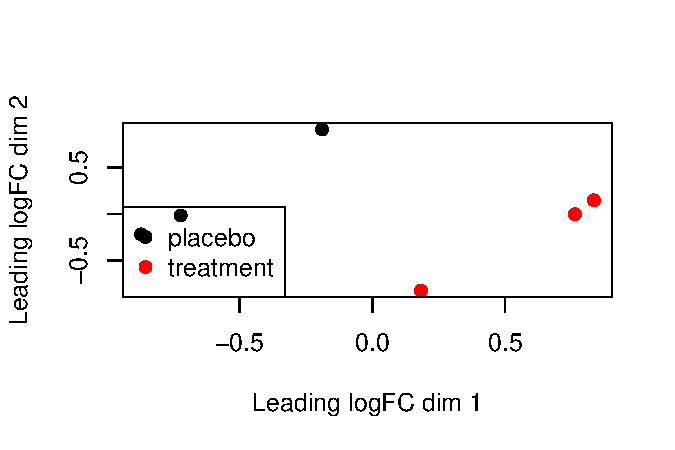
\includegraphics[width=\maxwidth]{figures/plots-edgeR-exploration-1} 

}



\end{knitrout}
\caption{Multi-dimensional scaling plot visualising the distance (log-fold expression) between the samples.}
\label{edgeR-mds}
\end{figure}



The estimation of the common and gene-specific dispersion factors is shown in figure \ref{edgeR-dispersion}. Note that the biological coefficient of variation is plotted, rather than the actual dispersion. 

% A mean variance plot is also provided in figure \ref{edgeR-ma}, which contrasts the raw, common, genewise and Poisson ($\mu = \sigma^2$) variances of the counts (code adapted from \textcite{ruddy_edger_2011}.

\begin{figure}[H]
  \centering
\begin{knitrout}
\definecolor{shadecolor}{rgb}{0.969, 0.969, 0.969}\color{fgcolor}

{\centering 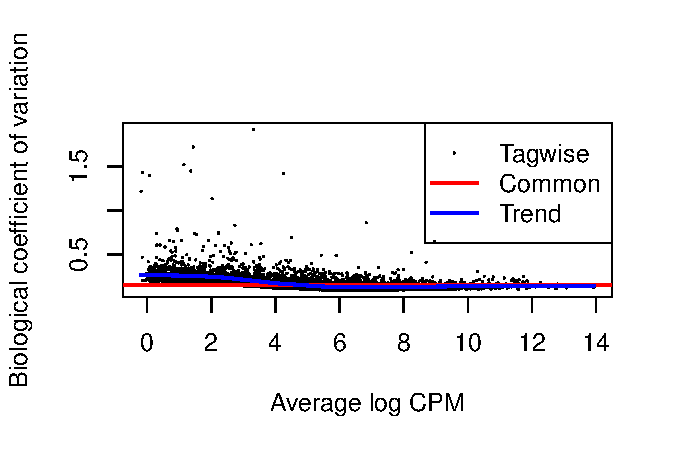
\includegraphics[width=\maxwidth]{figures/plots-edgeR-dispersion-plot-1} 

}



\end{knitrout}
\caption{Plot of the biological coefficient of variations (or the square root of the dispersion parameter of the NB model) for the common and tagwise method (trended method not relevant here). CPM = counts per million.}
\label{edgeR-dispersion}
\end{figure}
%' 
%' \begin{figure}[H]
%'   \centering
%' <<edgeR-dispersion-ma-plot, include=TRUE, results='hide',cache=TRUE, echo=FALSE,fig.width=6, fig.height=3.5,warning=F>>=
%' # code adapted from https://cgrlucb.wikispaces.com/file/view/edgeR_Tutorial.pdf
%' plotMeanVar( DEcounts , show.raw.vars=TRUE ,
%' show.tagwise.vars=TRUE ,
%' show.binned.common.disp.vars=FALSE ,
%' show.ave.raw.vars=FALSE ,
%' dispersion.method = "qcml" , NBline = TRUE ,
%' nbins = 100 ,
%' pch = 16 ,
%' xlab ="Mean Expression (Log10 Scale)" ,
%' ylab = "Variance (Log10 Scale)" ,
%' main = "Mean-Variance Plot" )
%' @
%' \caption{Mean-variance plot contrasting the raw, common, genewise and Poisson variances of the counts.}
%' \label{edgeR-ma}
%' \end{figure}



The top ten significant genes as found by the exact test are provided in table \ref{edgeR-top}. In total there are 704 genes significantly up- (372) or down- (332) regulated after controlling the FDR at 5\%. These genes are depicted in figure \ref{edgeR-de-genes} as the red dots. 

% latex table generated in R 3.2.3 by xtable 1.8-2 package
% Thu Mar 31 12:52:12 2016
\begin{table}[H]
\centering
\caption{Top ten differentially expressed genes
                            based on the edgeR exact test.} 
\label{edgeR-top}
\begin{tabular}{lrrr}
  \hline
Genes & logFC & PValue & FDR \\ 
  \hline
9831 & -4.60 & 0.00 & 0.00 \\ 
  2366 & 2.92 & 0.00 & 0.00 \\ 
  612 & -3.21 & 0.00 & 0.00 \\ 
  3192 & -2.20 & 0.00 & 0.00 \\ 
  6948 & -2.52 & 0.00 & 0.00 \\ 
  10305 & -4.11 & 0.00 & 0.00 \\ 
  6711 & -3.50 & 0.00 & 0.00 \\ 
  3411 & -2.45 & 0.00 & 0.00 \\ 
  30 & 2.78 & 0.00 & 0.00 \\ 
  6495 & -3.55 & 0.00 & 0.00 \\ 
   \hline
\end{tabular}
\end{table}


\begin{figure}[H]
  \centering
\begin{knitrout}
\definecolor{shadecolor}{rgb}{0.969, 0.969, 0.969}\color{fgcolor}

{\centering 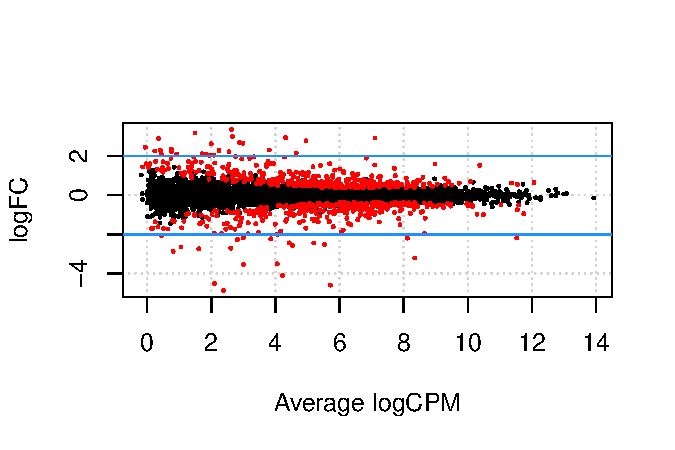
\includegraphics[width=\maxwidth]{figures/plots-edgeR-de-plot-1} 

}



\end{knitrout}
\caption{Plot of of the log-fold change against log-counts per million for edgeR. Significant genes (FDR 5\%) are highlighted in red. The blue lines indicate a log-fold change of two.}
\label{edgeR-de-genes}
\end{figure}

\subsection{Non-parametric - SAMSeq results}


We ran into a number of issues while performing the SAMSeq analysis. First, a 5\% FDR resulted in a set of significant genes that existed exclusively of up-regulated (filtered gene set) or down-regulated (unfiltered set) genes. After increasing the FDR to 20\%, this issue was resolved, but at the cost of many more false positives. 

Second, the four different options (FDR 5/20\% and an (un-)filtered dataset) resulted in extremely heterogeneous results (figure \ref{samseq-filterplot}). Only thirty-one significant genes were shared between the analyses. Even for the same FDR value, there were large discrepancies between the filtered and unfiltered results. At 20\% FDR, 64 of the filtered genes were still found to be significant (5 at 5\% FDR), while we would expect none of them to be significant due to the low counts. 

These large inconsistencies indicate that the SAMSeq method is not reliable for our dataset. We will discuss possible causes and solutions for these problems in the discussion section.

\begin{figure}[H]
\centering
\begin{knitrout}
\definecolor{shadecolor}{rgb}{0.969, 0.969, 0.969}\color{fgcolor}

{\centering 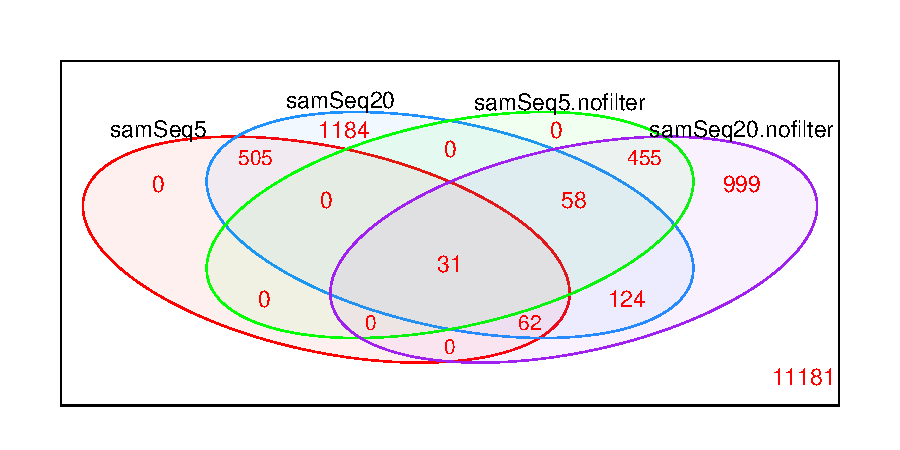
\includegraphics[width=\maxwidth]{figures/plots-samseq-plot-filter-1} 

}



\end{knitrout}
\caption{Venn diagram of the number of significant differentially expressed genes found by SAMSeq for an FDR of 5\% or 20 \% and using the entire or filtered dataset.}
\label{samseq-filterplot}
\end{figure}

% latex table generated in R 3.2.3 by xtable 1.8-2 package
% Thu Mar 31 12:16:52 2016
\begin{table}[H]
\centering
\caption{Top ten differentially expressed genes based on SAMSeq at 5\% (left) and 20\% FDR (right) respectively.} 
\label{samseq-table}
\begingroup\scriptsize
\begin{tabular}{llllll}
  \hline
Gene Name & Fold Change & q-value(\%) & Gene Name & Fold Change & q-value(\%) \\ 
  \hline
7 & 1.683 & 7.074 & 809 & 1.196 & 10.216 \\ 
  15 & 1.309 & 7.074 & 2400 & 1.4 & 10.216 \\ 
  16 & 6.222 & 7.074 & 4036 & 2.005 & 10.216 \\ 
  29 & 2.613 & 7.074 & 6225 & 1.192 & 10.216 \\ 
  35 & 1.426 & 7.074 & 6410 & 1.08 & 10.216 \\ 
  37 & 1.287 & 7.074 & 979 & 1.366 & 10.437 \\ 
  71 & 1.561 & 7.074 & 2679 & 1.156 & 10.437 \\ 
  91 & 1.362 & 7.074 & 4483 & 1.215 & 10.437 \\ 
  95 & 1.517 & 7.074 & 5325 & 1.279 & 10.437 \\ 
  103 & 1.536 & 7.074 & 53 & 0.782 & 10.653 \\ 
   \hline
\end{tabular}
\endgroup
\end{table}


For completeness, the top ten genes as reported by SAMSeq (after filtering), for 5 and 20\% FDR, are provided in table \ref{samseq-table}. Note that there were only 1 and 1964 unique q-values respectively, so the top ten genes are actually not that informative; all of the remaining genes are supposedly equally significant (in the case of 5\% FDR).

\subsection{Transformation - voom and limma results}



The mean-variance relation obtained by voom is shown in figure \ref{voom-var}. The top ten significant genes subsequently found by limma can be found in table \ref{limma-top}. In total there are 455 genes significantly up- (245) or down- (210) regulated when controlling the FDR at 5\%. A visual representation, similar to the one for EdgeR, is provided in figure \ref{limma-de-plot}.

\begin{figure}[H]
\centering
\begin{knitrout}
\definecolor{shadecolor}{rgb}{0.969, 0.969, 0.969}\color{fgcolor}

{\centering 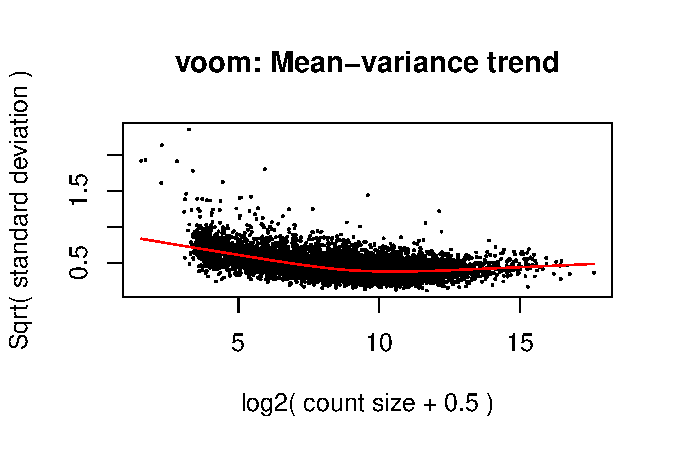
\includegraphics[width=\maxwidth]{figures/plots-voom-var-1} 

}



\end{knitrout}
\caption{Mean-variance relation estimated by voom.}
\label{voom-var}
\end{figure}

% latex table generated in R 3.2.3 by xtable 1.8-2 package
% Sun Mar 13 13:26:07 2016
\begin{table}[H]
\centering
\caption{Top ten differentially expressed genes
                            based on voom+limma.} 
\label{limma-top}
\begin{tabular}{lrrr}
  \hline
Genes & logFC & P.Value & FDR \\ 
  \hline
2366 & 2.94 & 0.00 & 0.00 \\ 
  612 & -3.17 & 0.00 & 0.00 \\ 
  9831 & -4.61 & 0.00 & 0.00 \\ 
  3192 & -2.20 & 0.00 & 0.00 \\ 
  6948 & -2.53 & 0.00 & 0.00 \\ 
  3411 & -2.42 & 0.00 & 0.00 \\ 
  30 & 2.79 & 0.00 & 0.00 \\ 
  11422 & 2.29 & 0.00 & 0.00 \\ 
  10305 & -4.11 & 0.00 & 0.00 \\ 
  6711 & -3.47 & 0.00 & 0.00 \\ 
   \hline
\end{tabular}
\end{table}


\begin{figure}[H]
\centering
\begin{knitrout}
\definecolor{shadecolor}{rgb}{0.969, 0.969, 0.969}\color{fgcolor}

{\centering 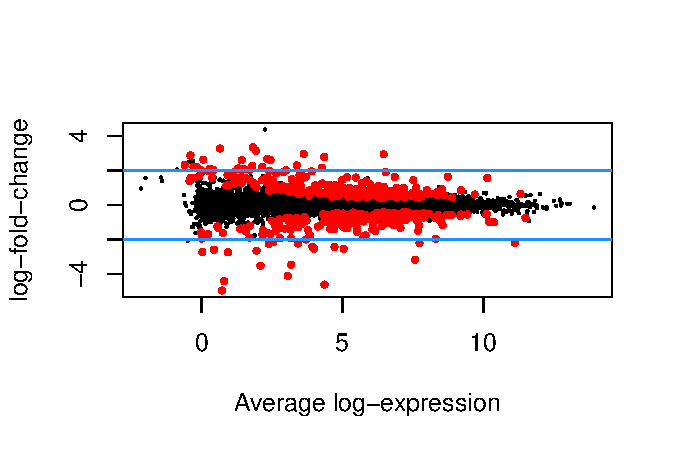
\includegraphics[width=\maxwidth]{figures/plots-voom-de-plot-1} 

}



\end{knitrout}
\caption{Plot of the log-fold change against log-counts per million for limma. Significant genes (FDR 5\%) are highlighted in red.}
\label{limma-de-plot}
\end{figure}

\subsection{Bayesian - EBSeq}


In total there were 423 genes that were found to be significantly up- or down-regulated when controlling the Bayesian FDR at 5\%. Almost all of these (412) had a posterior probability of one, so note that table \ref{EBSeq-top} is arbritrary in this sense, since the genes are merely sorted by their identifier.

% latex table generated in R 3.2.3 by xtable 1.8-2 package
% Sun Mar 13 13:26:47 2016
\begin{table}[H]
\centering
\caption{Top ten differentially expressed genes
                            based on EBSeq and their posterior probability of being differentially expressed.} 
\label{EBSeq-top}
\begin{tabular}{lr}
  \hline
Genes & Posterior P. DE \\ 
  \hline
8214 & 0.00 \\ 
  7617 & 0.00 \\ 
  831 & 0.00 \\ 
  10004 & 0.00 \\ 
  4508 & 0.00 \\ 
  11741 & 0.00 \\ 
  6240 & 0.00 \\ 
  1141 & 0.00 \\ 
  5697 & 0.00 \\ 
  6870 & 0.00 \\ 
   \hline
\end{tabular}
\end{table}


%' \begin{figure}[H]
%' \centering
%' <<ebseq-de-plot,include=TRUE, results='hide',cache=TRUE, echo=FALSE,fig.width=6, fig.height=4>>=
%' PlotPostVsRawFC(EBOut,PostFC(EBOut))
%' @
%' \caption{Mean-variance relation as estimated by voom.}
%' \label{ebseq-de-plot}
%' \end{figure}

\subsection{Agreement and differences between the methods}
The following Venn diagram depicts the overlap among the set of differentially expressed genes that were reported as significant by the four methods (figure \ref{venn-all}). Because the SAMSeq method was performing poorly and resulted in extremely different results, we also created an overlap plot for only edgeR, voom+limma and EBSeq (figure \ref{venn-simple}).

\begin{figure}[H]
\centering
\begin{knitrout}
\definecolor{shadecolor}{rgb}{0.969, 0.969, 0.969}\color{fgcolor}

{\centering 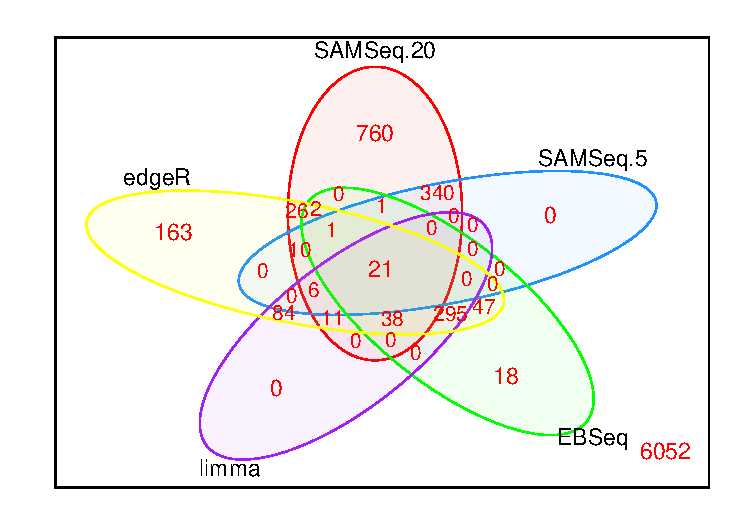
\includegraphics[width=\maxwidth]{figures/plots-venn-diagrams-1} 

}



\end{knitrout}
\caption{The number of significantly differentially expressed genes (either up- or down-regulated) for edgeR, voom+limma, EBSeq (FDR 5\%) and SAMSeq (FDR 5 or 20\%).}
\label{venn-all}
\end{figure}

\begin{figure}[H]
\centering
\begin{knitrout}
\definecolor{shadecolor}{rgb}{0.969, 0.969, 0.969}\color{fgcolor}

{\centering 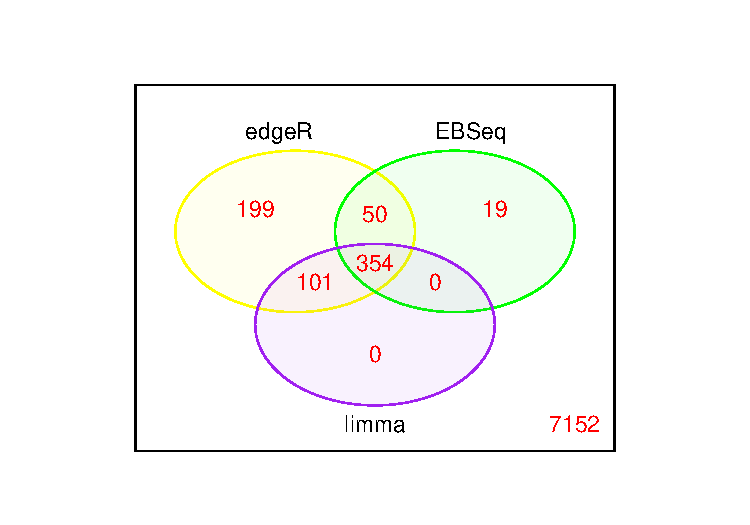
\includegraphics[width=\maxwidth]{figures/plots-venn-diagram-edge-limma-ebseq-1} 

}



\end{knitrout}
\caption{The number of significantly differentially expressed genes (either up- or down-regulated) at FDR 5\% for edgeR, voom+limma and EBSeq.}
\label{venn-simple}
\end{figure}

\section{Discussion}
The multidimensional scaling plot in figure \ref{edgeR-mds} indicates that the samples are reasonably well separated, although it seems that each group has one observation which behaves slightly differently (separation according to second axis).

Overall, there is quite a high degree of agreement between the parametric, Bayesian and transformation-based approaches (figure \ref{venn-simple}). This strengthens our confidence that the differentially expressed genes reported by these methods truly are so. We note that edgeR found 199 unique genes, whereas EBSeq only found 19 and limma did not find any. This might simply reflect the fact that edgeR reported almost half as many genes (704) as EBSeq (423) and limma (455). In the comparison by \textcite{soneson_comparison_2013} edgeR proved to be too liberal for small sample sizes as well. This is also, at least partly, consistent with the results of \textcite{seyednasrollah_comparison_2015}: in their simulation studies both edgeR and EBSeq proved to be too liberal and reported many more false positives than limma.

Looking at the top set of genes reported by edgeR (table \ref{edgeR-top}) and limma (table \ref{limma-top}), we see the same ones popping up. For EBSeq the list is a bit different (table \ref{EBSeq-top}), but this is an artefact of the internal sorting of the method, since a large portion of genes shared the same posterior probability.

% edgeR liberal for small samples soneson
% 
% SAMSeq: low power small sample sizes sonneseon + seyednasrollah
% 
% more replicates, differences between methods decrease \textcite{seyednasrollah_comparison_2015}.

The non-parametric SAMSeq method did not perform adequately in this analysis, but this was to be expected since it has poor power for small sample sizes \autocite{seyednasrollah_comparison_2015,soneson_comparison_2013}. However, it was still striking to observe that at a reasonable FDR cut-off of 5\%, the method reported only up- or down-regulated genes, but never both. This issue has since been addressed by one of the authors, in the form of another package npSeq \autocite{li2011using}. It implements the same methods that were described in the original SAMSeq paper \autocite{li_finding_2013}, but with symmetric, rather than asymmetric cut-offs for the non-parametric statistic. This could avoid the problem of exclusively finding up- or down-regulated genes, and instead find both simultaneously. Unfortunately this package was only available for Linux platforms at the time of writing, so we did not try it out.
Moreover, the fact that filtering had such a drastic effect on the called genes and that the overall agreement between different FDR cut-off values was so low, also shows how unstable this method was for our analysis (figure \ref{samseq-filterplot}). Lastly, we want to address our arbitrary choice of number of permutations and resampling rounds. We did not find any recommendations, apart from the default values implemented in the package. We increased these to be on the safe side, but a safer method would have been to slowly increase the number of simulations and evaluate when the results started to converge. 

The dangers of a low number of samples are not merely limited to the non-parametric method and we should be cautious for the other methods too. It is interesting that limma performs well in our dataset, despite the fact that it also suffers from low power for small sample sizes \autocite{soneson_comparison_2013}. The tendency of edgeR to be too liberal also decreases with growing sample size. 

% Finally, the discrete nature of the q-values, due to the permutation-based methods, also make it difficult to choose a reasonable top set of genes (since more genes than the intended number might share a q-value).

In general, all the methods become more similar and stable for increasing sample sizes \autocite{seyednasrollah_comparison_2015}. However, the optimal method still depends on the experimental conditions (heterogeneity of the sample, outliers, sample size) \autocite{soneson_comparison_2013}. The choice of method will also depend on the complexity of the experimental design. In this regard, the non-parametric SAMSeq method has an advantage, but limma and edgeR also offer support for this. Lastly, the final choice of method can in general be guided by practical issues as well, such as the availability of in-depth documentation and case-studies.

\clearpage
\printbibliography

\appendix
\section{Source code}
\begin{knitrout}
\definecolor{shadecolor}{rgb}{0.969, 0.969, 0.969}\color{fgcolor}\begin{kframe}
\begin{alltt}
\hlcom{# source('http://bioconductor.org/biocLite.R')}
\hlcom{# biocLite('edgeR')}
\hlkwd{library}\hlstd{(readxl)}
\hlstd{DEdata} \hlkwb{<-} \hlkwd{read_excel}\hlstd{(}\hlstr{"dataset.xlsx"}\hlstd{)}
\hlstd{DEdata} \hlkwb{<-} \hlstd{DEdata[,} \hlopt{-}\hlnum{1}\hlstd{]}
\hlstd{groupLabels} \hlkwb{<-} \hlkwd{c}\hlstd{(}\hlkwd{rep}\hlstd{(}\hlstr{"placebo"}\hlstd{,} \hlnum{3}\hlstd{),} \hlkwd{rep}\hlstd{(}\hlstr{"treatment"}\hlstd{,}
    \hlnum{3}\hlstd{))}
\hlcom{################################################# edgeR}
\hlkwd{library}\hlstd{(edgeR)}
\hlstd{DEcounts} \hlkwb{<-} \hlkwd{DGEList}\hlstd{(}\hlkwc{counts} \hlstd{= DEdata,} \hlkwc{group} \hlstd{=} \hlkwd{factor}\hlstd{(groupLabels))}
\hlstd{DEcounts.original} \hlkwb{<-} \hlstd{DEcounts}
\hlcom{# filtering relative to library size}
\hlstd{keep} \hlkwb{<-} \hlkwd{rowSums}\hlstd{(}\hlkwd{cpm}\hlstd{(DEcounts)} \hlopt{>} \hlnum{1}\hlstd{)} \hlopt{>=} \hlnum{3}  \hlcom{# 1 read per million for at least 3 samples}
\hlstd{DEcounts} \hlkwb{<-} \hlstd{DEcounts[keep, ,} \hlkwc{keep.lib.sizes} \hlstd{=} \hlnum{FALSE}\hlstd{]}
\hlstd{DEcounts}\hlopt{$}\hlstd{samples}\hlopt{$}\hlstd{lib.size} \hlkwb{<-} \hlkwd{colSums}\hlstd{(DEcounts}\hlopt{$}\hlstd{counts)}  \hlcom{# recompute library sizes}
\hlcom{# How many tags were removed?}
\hlstd{ntags.filtered} \hlkwb{<-} \hlkwd{dim}\hlstd{(DEcounts)[}\hlnum{1}\hlstd{]}
\hlstd{ntags.original} \hlkwb{<-} \hlkwd{dim}\hlstd{(DEcounts.original)[}\hlnum{1}\hlstd{]}
\hlcom{# trimmed mean of M-values (TMM)}
\hlcom{# normalisation for sample}
\hlcom{# specific-effects - MODEL BASED not a}
\hlcom{# transformation!}
\hlstd{DEcounts} \hlkwb{<-} \hlkwd{calcNormFactors}\hlstd{(DEcounts,} \hlkwc{method} \hlstd{=} \hlstr{"TMM"}\hlstd{)}
\hlcom{# smear plot before and after correction}
\hlkwd{par}\hlstd{(}\hlkwc{mfrow} \hlstd{=} \hlkwd{c}\hlstd{(}\hlnum{1}\hlstd{,} \hlnum{2}\hlstd{))}
\hlkwd{maPlot}\hlstd{(DEcounts}\hlopt{$}\hlstd{counts[,} \hlnum{1}\hlstd{], DEcounts}\hlopt{$}\hlstd{counts[,}
    \hlnum{4}\hlstd{],} \hlkwc{normalise} \hlstd{=} \hlnum{TRUE}\hlstd{,} \hlkwc{pch} \hlstd{=} \hlnum{19}\hlstd{,} \hlkwc{cex} \hlstd{=} \hlnum{0.4}\hlstd{,}
    \hlkwc{ylim} \hlstd{=} \hlkwd{c}\hlstd{(}\hlopt{-}\hlnum{8}\hlstd{,} \hlnum{8}\hlstd{))}
\hlkwd{grid}\hlstd{(}\hlkwc{col} \hlstd{=} \hlstr{"blue"}\hlstd{)}
\hlkwd{abline}\hlstd{(}\hlkwc{h} \hlstd{=} \hlkwd{log2}\hlstd{(DEcounts}\hlopt{$}\hlstd{samples}\hlopt{$}\hlstd{norm.factors[}\hlnum{2}\hlstd{]}\hlopt{/}\hlstd{DEcounts}\hlopt{$}\hlstd{samples}\hlopt{$}\hlstd{norm.factors[}\hlnum{1}\hlstd{]),}
    \hlkwc{col} \hlstd{=} \hlstr{"red"}\hlstd{,} \hlkwc{lwd} \hlstd{=} \hlnum{4}\hlstd{)}
\hlstd{eff.libsize} \hlkwb{<-} \hlstd{DEcounts}\hlopt{$}\hlstd{samples}\hlopt{$}\hlstd{lib.size} \hlopt{*}
    \hlstd{DEcounts}\hlopt{$}\hlstd{samples}\hlopt{$}\hlstd{norm.factors}
\hlkwd{maPlot}\hlstd{(DEcounts}\hlopt{$}\hlstd{counts[,} \hlnum{1}\hlstd{]}\hlopt{/}\hlstd{eff.libsize[}\hlnum{1}\hlstd{],}
    \hlstd{DEcounts}\hlopt{$}\hlstd{counts[,} \hlnum{2}\hlstd{]}\hlopt{/}\hlstd{eff.libsize[}\hlnum{2}\hlstd{],}
    \hlkwc{normalise} \hlstd{=} \hlnum{FALSE}\hlstd{,} \hlkwc{pch} \hlstd{=} \hlnum{19}\hlstd{,} \hlkwc{cex} \hlstd{=} \hlnum{0.4}\hlstd{,}
    \hlkwc{ylim} \hlstd{=} \hlkwd{c}\hlstd{(}\hlopt{-}\hlnum{8}\hlstd{,} \hlnum{8}\hlstd{))}
\hlkwd{grid}\hlstd{(}\hlkwc{col} \hlstd{=} \hlstr{"blue"}\hlstd{)}
\hlkwd{par}\hlstd{(}\hlkwc{mfrow} \hlstd{=} \hlkwd{c}\hlstd{(}\hlnum{1}\hlstd{,} \hlnum{1}\hlstd{))}
\hlkwd{plotMDS}\hlstd{(DEcounts,} \hlkwc{col} \hlstd{=} \hlkwd{as.numeric}\hlstd{(DEcounts}\hlopt{$}\hlstd{samples}\hlopt{$}\hlstd{group),}
    \hlkwc{pch} \hlstd{=} \hlnum{19}\hlstd{)}
\hlkwd{legend}\hlstd{(}\hlstr{"bottomleft"}\hlstd{,} \hlkwd{as.character}\hlstd{(}\hlkwd{unique}\hlstd{(DEcounts}\hlopt{$}\hlstd{samples}\hlopt{$}\hlstd{group)),}
    \hlkwc{col} \hlstd{=} \hlnum{1}\hlopt{:}\hlnum{2}\hlstd{,} \hlkwc{pch} \hlstd{=} \hlnum{19}\hlstd{)}
\hlcom{# Negative Binomial model}
\hlstd{DEcounts} \hlkwb{<-} \hlkwd{estimateDisp}\hlstd{(DEcounts)}
\hlkwd{plotBCV}\hlstd{(DEcounts)}  \hlcom{# dispersion estimation}
\hlstd{et} \hlkwb{<-} \hlkwd{exactTest}\hlstd{(DEcounts,} \hlkwc{dispersion} \hlstd{=} \hlstr{"tagwise"}\hlstd{,}
    \hlkwc{rejection.region} \hlstd{=} \hlstr{"deviance"}\hlstd{)}
\hlcom{# deviance slightly less conservative,}
\hlcom{# conditional likelihood ratio test}
\hlstd{edge.top} \hlkwb{<-} \hlkwd{topTags}\hlstd{(et,} \hlkwc{n} \hlstd{=} \hlnum{10}\hlstd{,} \hlkwc{adjust.method} \hlstd{=} \hlstr{"BH"}\hlstd{)}  \hlcom{#  false discovery rate, }
\hlcom{# = the expected proportion of false}
\hlcom{# discoveries amongst the rejected}
\hlcom{# hypotheses}
\hlkwd{library}\hlstd{(xtable)}
\hlstd{toptable} \hlkwb{<-} \hlkwd{as.data.frame}\hlstd{(edge.top[,} \hlopt{-}\hlnum{2}\hlstd{])}
\hlstd{toptable} \hlkwb{<-} \hlkwd{cbind}\hlstd{(}\hlkwd{rownames}\hlstd{(toptable), toptable)}
\hlkwd{colnames}\hlstd{(toptable)[}\hlnum{1}\hlstd{]} \hlkwb{<-} \hlstr{"Genes"}
\hlstd{tab} \hlkwb{<-} \hlkwd{xtable}\hlstd{(toptable,} \hlkwc{booktabs} \hlstd{= T,} \hlkwc{caption} \hlstd{=} \hlkwd{paste}\hlstd{(}\hlstr{"Top ten differentially expressed genes\textbackslash{}n                            based on the edgeR exact test."}\hlstd{),}
    \hlkwc{label} \hlstd{=} \hlstr{"edgeR-top"}\hlstd{)}
\hlkwd{print}\hlstd{(tab,} \hlkwc{caption.placement} \hlstd{=} \hlstr{"top"}\hlstd{,} \hlkwc{table.placement} \hlstd{=} \hlstr{"H"}\hlstd{,}
    \hlkwc{include.rownames} \hlstd{= F)}
\hlcom{# # Show counts for top 10 genes o <-}
\hlcom{# order(et$table$PValue)}
\hlcom{# cpm(DEcounts)[o[1:10],]}
\hlcom{# total number of differentially}
\hlcom{# expressed genes at FDR 5%}
\hlstd{sign.genes.edger} \hlkwb{<-} \hlkwd{summary}\hlstd{(de} \hlkwb{<-} \hlkwd{decideTestsDGE}\hlstd{(et,}
    \hlkwc{adjust.method} \hlstd{=} \hlstr{"BH"}\hlstd{,} \hlkwc{p.value} \hlstd{=} \hlnum{0.05}\hlstd{))}
\hlcom{# gene namelist}
\hlstd{genelist.edger} \hlkwb{<-} \hlkwd{rownames}\hlstd{(DEdata[keep, ][de} \hlopt{==}
    \hlnum{1} \hlopt{|} \hlstd{de} \hlopt{== -}\hlnum{1}\hlstd{, ])}
\hlcom{# Plot log-fold change against log-counts}
\hlcom{# per million - DE genes highlighted:}
\hlstd{detags} \hlkwb{<-} \hlkwd{rownames}\hlstd{(DEcounts)[}\hlkwd{as.logical}\hlstd{(de)]}
\hlkwd{plotSmear}\hlstd{(et,} \hlkwc{de.tags} \hlstd{= detags)}
\hlkwd{abline}\hlstd{(}\hlkwc{h} \hlstd{=} \hlkwd{c}\hlstd{(}\hlopt{-}\hlnum{2}\hlstd{,} \hlnum{2}\hlstd{),} \hlkwc{col} \hlstd{=} \hlstr{"dodgerblue"}\hlstd{)}
\hlcom{################################################# SAMSeq}
\hlkwd{library}\hlstd{(samr)}
\hlstd{samfit.5} \hlkwb{<-} \hlkwd{SAMseq}\hlstd{(}\hlkwc{x} \hlstd{= DEdata[keep, ],} \hlkwc{y} \hlstd{=} \hlkwd{c}\hlstd{(}\hlkwd{rep}\hlstd{(}\hlstr{"1"}\hlstd{,}
    \hlnum{3}\hlstd{),} \hlkwd{rep}\hlstd{(}\hlstr{"2"}\hlstd{,} \hlnum{3}\hlstd{)),} \hlkwc{resp.type} \hlstd{=} \hlstr{"Two class unpaired"}\hlstd{,}
    \hlkwc{nperms} \hlstd{=} \hlnum{500}\hlstd{,} \hlkwc{random.seed} \hlstd{=} \hlnum{43893}\hlstd{,} \hlkwc{nresamp} \hlstd{=} \hlnum{100}\hlstd{,}
    \hlkwc{fdr.output} \hlstd{=} \hlnum{0.05}\hlstd{)}
\hlkwd{plot}\hlstd{(samfit.5)}
\hlstd{samfit.5.nofilter} \hlkwb{<-} \hlkwd{SAMseq}\hlstd{(}\hlkwc{x} \hlstd{= DEdata,} \hlkwc{y} \hlstd{=} \hlkwd{c}\hlstd{(}\hlkwd{rep}\hlstd{(}\hlstr{"1"}\hlstd{,}
    \hlnum{3}\hlstd{),} \hlkwd{rep}\hlstd{(}\hlstr{"2"}\hlstd{,} \hlnum{3}\hlstd{)),} \hlkwc{resp.type} \hlstd{=} \hlstr{"Two class unpaired"}\hlstd{,}
    \hlkwc{nperms} \hlstd{=} \hlnum{500}\hlstd{,} \hlkwc{random.seed} \hlstd{=} \hlnum{43893}\hlstd{,} \hlkwc{nresamp} \hlstd{=} \hlnum{100}\hlstd{,}
    \hlkwc{fdr.output} \hlstd{=} \hlnum{0.05}\hlstd{)}
\hlkwd{plot}\hlstd{(samfit.5.nofilter)}
\hlstd{samfit.20} \hlkwb{<-} \hlkwd{SAMseq}\hlstd{(}\hlkwc{x} \hlstd{= DEdata[keep, ],} \hlkwc{y} \hlstd{=} \hlkwd{c}\hlstd{(}\hlkwd{rep}\hlstd{(}\hlstr{"1"}\hlstd{,}
    \hlnum{3}\hlstd{),} \hlkwd{rep}\hlstd{(}\hlstr{"2"}\hlstd{,} \hlnum{3}\hlstd{)),} \hlkwc{resp.type} \hlstd{=} \hlstr{"Two class unpaired"}\hlstd{,}
    \hlkwc{nperms} \hlstd{=} \hlnum{500}\hlstd{,} \hlkwc{random.seed} \hlstd{=} \hlnum{43893}\hlstd{,} \hlkwc{nresamp} \hlstd{=} \hlnum{100}\hlstd{,}
    \hlkwc{fdr.output} \hlstd{=} \hlnum{0.2}\hlstd{)}
\hlkwd{print}\hlstd{(samfit.20)}
\hlkwd{plot}\hlstd{(samfit.20)}
\hlstd{samfit.20.nofilter} \hlkwb{<-} \hlkwd{SAMseq}\hlstd{(}\hlkwc{x} \hlstd{= DEdata,}
    \hlkwc{y} \hlstd{=} \hlkwd{c}\hlstd{(}\hlkwd{rep}\hlstd{(}\hlstr{"1"}\hlstd{,} \hlnum{3}\hlstd{),} \hlkwd{rep}\hlstd{(}\hlstr{"2"}\hlstd{,} \hlnum{3}\hlstd{)),} \hlkwc{resp.type} \hlstd{=} \hlstr{"Two class unpaired"}\hlstd{,}
    \hlkwc{nperms} \hlstd{=} \hlnum{500}\hlstd{,} \hlkwc{random.seed} \hlstd{=} \hlnum{43893}\hlstd{,} \hlkwc{nresamp} \hlstd{=} \hlnum{100}\hlstd{,}
    \hlkwc{fdr.output} \hlstd{=} \hlnum{0.2}\hlstd{)}
\hlkwd{plot}\hlstd{(samfit.20.nofilter)}
\hlcom{# retrieve list of significant gene names}
\hlstd{genelist.samseq.5} \hlkwb{<-} \hlkwd{c}\hlstd{(samfit.5}\hlopt{$}\hlstd{siggenes.table}\hlopt{$}\hlstd{genes.up[,}
    \hlnum{2}\hlstd{], samfit.5}\hlopt{$}\hlstd{siggenes.table}\hlopt{$}\hlstd{genes.lo[,}
    \hlnum{2}\hlstd{])}
\hlstd{genelist.samseq.5.nofilter} \hlkwb{<-} \hlkwd{c}\hlstd{(samfit.5.nofilter}\hlopt{$}\hlstd{siggenes.table}\hlopt{$}\hlstd{genes.up[,}
    \hlnum{2}\hlstd{], samfit.5.nofilter}\hlopt{$}\hlstd{siggenes.table}\hlopt{$}\hlstd{genes.lo[,}
    \hlnum{2}\hlstd{])}
\hlstd{genelist.samseq.20} \hlkwb{<-} \hlkwd{c}\hlstd{(samfit.20}\hlopt{$}\hlstd{siggenes.table}\hlopt{$}\hlstd{genes.up[,}
    \hlnum{2}\hlstd{], samfit.20}\hlopt{$}\hlstd{siggenes.table}\hlopt{$}\hlstd{genes.lo[,}
    \hlnum{2}\hlstd{])}
\hlstd{genelist.samseq.20.nofilter} \hlkwb{<-} \hlkwd{c}\hlstd{(samfit.20.nofilter}\hlopt{$}\hlstd{siggenes.table}\hlopt{$}\hlstd{genes.up[,}
    \hlnum{2}\hlstd{], samfit.20.nofilter}\hlopt{$}\hlstd{siggenes.table}\hlopt{$}\hlstd{genes.lo[,}
    \hlnum{2}\hlstd{])}
\hlcom{# create testresults matrix-like object}
\hlcom{# for limma venn diagrams (can decidetest}
\hlcom{# be used on samseq output to make this}
\hlcom{# easier?)  dont use DEdata[keep,]}
\hlcom{# because then we cant compare filtered}
\hlcom{# and unfiltered sets}
\hlstd{sam.5.testresults} \hlkwb{<-} \hlkwd{sapply}\hlstd{(}\hlkwd{rownames}\hlstd{(DEdata),}
    \hlkwa{function}\hlstd{(}\hlkwc{x}\hlstd{)} \hlkwd{ifelse}\hlstd{(x} \hlopt \hlstd{genelist.samseq.5,}
        \hlnum{1}\hlstd{,} \hlnum{0}\hlstd{))}
\hlstd{sam.5.nofilter.testresults} \hlkwb{<-} \hlkwd{sapply}\hlstd{(}\hlkwd{rownames}\hlstd{(DEdata),}
    \hlkwa{function}\hlstd{(}\hlkwc{x}\hlstd{)} \hlkwd{ifelse}\hlstd{(x} \hlopt \hlstd{genelist.samseq.5.nofilter,}
        \hlnum{1}\hlstd{,} \hlnum{0}\hlstd{))}
\hlstd{sam.20.testresults} \hlkwb{<-} \hlkwd{sapply}\hlstd{(}\hlkwd{rownames}\hlstd{(DEdata),}
    \hlkwa{function}\hlstd{(}\hlkwc{x}\hlstd{)} \hlkwd{ifelse}\hlstd{(x} \hlopt \hlstd{genelist.samseq.20,}
        \hlnum{1}\hlstd{,} \hlnum{0}\hlstd{))}
\hlstd{sam.20.nofilter.testresults} \hlkwb{<-} \hlkwd{sapply}\hlstd{(}\hlkwd{rownames}\hlstd{(DEdata),}
    \hlkwa{function}\hlstd{(}\hlkwc{x}\hlstd{)} \hlkwd{ifelse}\hlstd{(x} \hlopt \hlstd{genelist.samseq.20.nofilter,}
        \hlnum{1}\hlstd{,} \hlnum{0}\hlstd{))}
\hlcom{# How many filtered genes were called as}
\hlcom{# significant?}
\hlstd{filtered.genelist} \hlkwb{<-} \hlkwd{rownames}\hlstd{(DEdata[}\hlopt{!}\hlstd{keep,}
    \hlstd{])}
\hlstd{sig.filter.5} \hlkwb{<-} \hlkwd{sum}\hlstd{(}\hlkwd{sapply}\hlstd{(filtered.genelist,}
    \hlkwa{function}\hlstd{(}\hlkwc{x}\hlstd{) x} \hlopt \hlstd{genelist.samseq.5.nofilter))}
\hlstd{sig.filter.20} \hlkwb{<-} \hlkwd{sum}\hlstd{(}\hlkwd{sapply}\hlstd{(filtered.genelist,}
    \hlkwa{function}\hlstd{(}\hlkwc{x}\hlstd{) x} \hlopt \hlstd{genelist.samseq.20.nofilter))}
\hlcom{# Comparison between filtered and}
\hlcom{# unfiltered SAMSeq analysis}
\hlstd{sam5.vs.nofilter} \hlkwb{<-} \hlkwd{cbind}\hlstd{(}\hlkwc{sam5nofilter} \hlstd{= sam.5.nofilter.testresults,}
    \hlkwc{sam5} \hlstd{= sam.5.testresults)}
\hlstd{sam20.vs.nofilter} \hlkwb{<-} \hlkwd{cbind}\hlstd{(}\hlkwc{sam20nofilter} \hlstd{= sam.20.nofilter.testresults,}
    \hlkwc{sam5} \hlstd{= sam.20.testresults)}
\hlstd{sam5.vs.sam20} \hlkwb{<-} \hlkwd{cbind}\hlstd{(}\hlkwc{sam20} \hlstd{= sam.20.testresults,}
    \hlkwc{sam5} \hlstd{= sam.5.testresults)}
\hlkwd{vennCounts}\hlstd{(sam5.vs.nofilter)}
\hlkwd{vennCounts}\hlstd{(sam20.vs.nofilter)}
\hlkwd{vennCounts}\hlstd{(sam5.vs.sam20)}
\hlcom{# sum(is.element(genelist.samseq,genelist.edger))}
\hlkwd{vennDiagram}\hlstd{(}\hlkwd{vennCounts}\hlstd{(}\hlkwd{cbind}\hlstd{(}\hlkwc{samSeq5} \hlstd{= sam.5.testresults,}
    \hlkwc{samSeq20} \hlstd{= sam.20.testresults,} \hlkwc{samSeq5.nofilter} \hlstd{= sam.5.nofilter.testresults,}
    \hlkwc{samSeq20.nofilter} \hlstd{= sam.20.nofilter.testresults)),}
    \hlkwc{include} \hlstd{=} \hlstr{"both"}\hlstd{,} \hlkwc{counts.col} \hlstd{=} \hlkwd{c}\hlstd{(}\hlstr{"red"}\hlstd{,}
        \hlstr{"dodgerblue"}\hlstd{),} \hlkwc{circle.col} \hlstd{=} \hlkwd{c}\hlstd{(}\hlstr{"red"}\hlstd{,}
        \hlstr{"dodgerblue"}\hlstd{,} \hlstr{"green"}\hlstd{,} \hlstr{"purple"}\hlstd{))}
\hlcom{# Comparing SAMSeq with edgeR need to use}
\hlcom{# DEdata[keep,] for comparison with edgeR}
\hlstd{sam.5.testresults.filter} \hlkwb{<-} \hlkwd{sapply}\hlstd{(}\hlkwd{rownames}\hlstd{(DEdata[keep,}
    \hlstd{]),} \hlkwa{function}\hlstd{(}\hlkwc{x}\hlstd{)} \hlkwd{ifelse}\hlstd{(x} \hlopt \hlstd{genelist.samseq.5,}
    \hlnum{1}\hlstd{,} \hlnum{0}\hlstd{))}
\hlstd{sam.20.testresults.filter} \hlkwb{<-} \hlkwd{sapply}\hlstd{(}\hlkwd{rownames}\hlstd{(DEdata[keep,}
    \hlstd{]),} \hlkwa{function}\hlstd{(}\hlkwc{x}\hlstd{)} \hlkwd{ifelse}\hlstd{(x} \hlopt \hlstd{genelist.samseq.20,}
    \hlnum{1}\hlstd{,} \hlnum{0}\hlstd{))}
\hlstd{edger.vs.samseq.5} \hlkwb{<-} \hlkwd{cbind}\hlstd{(}\hlkwc{edgeR} \hlstd{=} \hlkwd{as.numeric}\hlstd{(de}\hlopt{@}\hlkwc{.Data}\hlstd{),}
    \hlkwc{samSeq5} \hlstd{= sam.5.testresults.filter)}
\hlstd{edger.vs.samseq.20} \hlkwb{<-} \hlkwd{cbind}\hlstd{(}\hlkwc{edgeR} \hlstd{=} \hlkwd{as.numeric}\hlstd{(de}\hlopt{@}\hlkwc{.Data}\hlstd{),}
    \hlkwc{samSeq20} \hlstd{= sam.20.testresults.filter)}
\hlcom{# Venn diagram counts}
\hlkwd{vennCounts}\hlstd{(edger.vs.samseq.5)}
\hlkwd{vennCounts}\hlstd{(edger.vs.samseq.20)}
\hlkwd{vennDiagram}\hlstd{(}\hlkwd{vennCounts}\hlstd{(edger.vs.samseq.5),}
    \hlkwc{include} \hlstd{=} \hlstr{"both"}\hlstd{,} \hlkwc{counts.col} \hlstd{=} \hlkwd{c}\hlstd{(}\hlstr{"red"}\hlstd{,}
        \hlstr{"dodgerblue"}\hlstd{),} \hlkwc{circle.col} \hlstd{=} \hlkwd{c}\hlstd{(}\hlstr{"red"}\hlstd{,}
        \hlstr{"dodgerblue"}\hlstd{,} \hlstr{"green"}\hlstd{))}
\hlkwd{vennDiagram}\hlstd{(}\hlkwd{vennCounts}\hlstd{(edger.vs.samseq.20),}
    \hlkwc{include} \hlstd{=} \hlstr{"both"}\hlstd{,} \hlkwc{counts.col} \hlstd{=} \hlkwd{c}\hlstd{(}\hlstr{"red"}\hlstd{,}
        \hlstr{"dodgerblue"}\hlstd{),} \hlkwc{circle.col} \hlstd{=} \hlkwd{c}\hlstd{(}\hlstr{"red"}\hlstd{,}
        \hlstr{"dodgerblue"}\hlstd{,} \hlstr{"green"}\hlstd{))}
\hlcom{# npseq symmetric cutoffs, not available}
\hlcom{# in windows?}
\hlkwd{vennDiagram}\hlstd{(}\hlkwd{vennCounts}\hlstd{(}\hlkwd{cbind}\hlstd{(}\hlkwc{samSeq5} \hlstd{= sam.5.testresults,}
    \hlkwc{samSeq20} \hlstd{= sam.20.testresults,} \hlkwc{samSeq5.nofilter} \hlstd{= sam.5.nofilter.testresults,}
    \hlkwc{samSeq20.nofilter} \hlstd{= sam.20.nofilter.testresults)),}
    \hlkwc{include} \hlstd{=} \hlstr{"both"}\hlstd{,} \hlkwc{cex} \hlstd{=} \hlkwd{c}\hlstd{(}\hlnum{0.9}\hlstd{,} \hlnum{0.9}\hlstd{,} \hlnum{0.8}\hlstd{),}
    \hlkwc{counts.col} \hlstd{=} \hlkwd{c}\hlstd{(}\hlstr{"red"}\hlstd{,} \hlstr{"dodgerblue"}\hlstd{),}
    \hlkwc{circle.col} \hlstd{=} \hlkwd{c}\hlstd{(}\hlstr{"red"}\hlstd{,} \hlstr{"dodgerblue"}\hlstd{,} \hlstr{"green"}\hlstd{,}
        \hlstr{"purple"}\hlstd{))}
\hlstd{samseq.5.table} \hlkwb{<-} \hlkwd{as.data.frame}\hlstd{(}\hlkwd{rbind}\hlstd{(samfit.5}\hlopt{$}\hlstd{siggenes.table}\hlopt{$}\hlstd{genes.up,}
    \hlstd{samfit.5}\hlopt{$}\hlstd{siggenes.table}\hlopt{$}\hlstd{genes.lo))}
\hlstd{samseq.5.table} \hlkwb{<-} \hlstd{samseq.5.table[}\hlkwd{order}\hlstd{(samseq.5.table}\hlopt{$}\hlstd{`q-value(%)`),}
    \hlstd{]}
\hlcom{# length(unique(samseq.5.table$`q-value(%)`))}
\hlcom{# length(samseq.5.table$`q-value(%)`)}
\hlstd{samseq.20.table} \hlkwb{<-} \hlkwd{as.data.frame}\hlstd{(}\hlkwd{rbind}\hlstd{(samfit.20}\hlopt{$}\hlstd{siggenes.table}\hlopt{$}\hlstd{genes.up,}
    \hlstd{samfit.20}\hlopt{$}\hlstd{siggenes.table}\hlopt{$}\hlstd{genes.lo))}
\hlstd{samseq.20.table} \hlkwb{<-} \hlstd{samseq.20.table[}\hlkwd{order}\hlstd{(samseq.20.table}\hlopt{$}\hlstd{`q-value(%)`),}
    \hlstd{]}
\hlcom{# length(unique(samseq.20.table$`q-value(%)`))}
\hlstd{unique.20} \hlkwb{<-} \hlkwd{length}\hlstd{(samseq.20.table}\hlopt{$}\hlstd{`q-value(%)`)}
\hlstd{samseqtable} \hlkwb{<-} \hlkwd{xtable}\hlstd{(}\hlkwd{cbind}\hlstd{(samseq.5.table[}\hlnum{1}\hlopt{:}\hlnum{10}\hlstd{,}
    \hlopt{-}\hlkwd{c}\hlstd{(}\hlnum{1}\hlstd{,} \hlnum{3}\hlstd{)], samseq.20.table[}\hlnum{1}\hlopt{:}\hlnum{10}\hlstd{,} \hlopt{-}\hlkwd{c}\hlstd{(}\hlnum{1}\hlstd{,}
    \hlnum{3}\hlstd{)]),} \hlkwc{include.rownames} \hlstd{= F,} \hlkwc{booktabs} \hlstd{= T,}
    \hlkwc{caption} \hlstd{=} \hlkwd{paste}\hlstd{(}\hlstr{"Top ten differentially expressed genes based on SAMSeq at 5\textbackslash{}\textbackslash{}% (left) and 20\textbackslash{}\textbackslash{}% FDR (right) respectively."}\hlstd{),}
    \hlkwc{label} \hlstd{=} \hlstr{"samseq-table"}\hlstd{)}
\hlkwd{print}\hlstd{(samseqtable,} \hlkwc{caption.placement} \hlstd{=} \hlstr{"top"}\hlstd{,}
    \hlkwc{table.placement} \hlstd{=} \hlstr{"H"}\hlstd{,} \hlkwc{size} \hlstd{=} \hlstr{"scriptsize"}\hlstd{,}
    \hlkwc{include.rownames} \hlstd{= F)}
\hlcom{################################################# limma + voom}
\hlkwd{library}\hlstd{(limma)}
\hlstd{dge} \hlkwb{<-} \hlkwd{DGEList}\hlstd{(}\hlkwc{counts} \hlstd{= DEdata,} \hlkwc{group} \hlstd{=} \hlkwd{factor}\hlstd{(groupLabels))}
\hlstd{dge} \hlkwb{<-} \hlstd{dge[keep, ,} \hlkwc{keep.lib.sizes} \hlstd{=} \hlnum{FALSE}\hlstd{]}  \hlcom{# filter}
\hlstd{dge}\hlopt{$}\hlstd{samples}\hlopt{$}\hlstd{lib.size} \hlkwb{<-} \hlkwd{colSums}\hlstd{(dge}\hlopt{$}\hlstd{counts)}  \hlcom{# recompute library sizes}
\hlstd{dge} \hlkwb{<-} \hlkwd{calcNormFactors}\hlstd{(dge,} \hlkwc{method} \hlstd{=} \hlstr{"TMM"}\hlstd{)}  \hlcom{# normalisation}
\hlcom{# voom transform}
\hlstd{design} \hlkwb{<-} \hlkwd{model.matrix}\hlstd{(}\hlopt{~}\hlkwd{as.factor}\hlstd{(groupLabels))}
\hlstd{v} \hlkwb{<-} \hlkwd{voom}\hlstd{(dge, design,} \hlkwc{plot} \hlstd{=} \hlnum{TRUE}\hlstd{)}
\hlkwd{plotMDS}\hlstd{(v)}
\hlcom{# limma model}
\hlstd{fit} \hlkwb{<-} \hlkwd{lmFit}\hlstd{(v, design)}
\hlstd{fit} \hlkwb{<-} \hlkwd{eBayes}\hlstd{(fit)}
\hlcom{# top ten genes}
\hlstd{limma.top} \hlkwb{<-} \hlkwd{topTable}\hlstd{(fit,} \hlkwc{coef} \hlstd{=} \hlkwd{ncol}\hlstd{(design),}
    \hlkwc{adjust.method} \hlstd{=} \hlstr{"BH"}\hlstd{,} \hlkwc{number} \hlstd{=} \hlnum{10}\hlstd{)}
\hlcom{# number of significant genes}
\hlstd{all.limma} \hlkwb{<-} \hlkwd{topTable}\hlstd{(fit,} \hlkwc{coef} \hlstd{=} \hlkwd{ncol}\hlstd{(design),}
    \hlkwc{adjust.method} \hlstd{=} \hlstr{"BH"}\hlstd{,} \hlkwc{number} \hlstd{=} \hlkwd{dim}\hlstd{(dge}\hlopt{$}\hlstd{counts)[}\hlnum{1}\hlstd{])}
\hlstd{sign.limma} \hlkwb{<-} \hlstd{all.limma[all.limma}\hlopt{$}\hlstd{adj.P.Val} \hlopt{<}
    \hlnum{0.05}\hlstd{, ]}
\hlkwd{dim}\hlstd{(sign.limma)[}\hlnum{1}\hlstd{]}
\hlcom{# or look at treatment effect (ignore}
\hlcom{# intercept)}
\hlstd{sign.genes.limma} \hlkwb{<-} \hlkwd{summary}\hlstd{(de.limma} \hlkwb{<-} \hlkwd{decideTests}\hlstd{(fit,}
    \hlkwc{adjust.method} \hlstd{=} \hlstr{"BH"}\hlstd{,} \hlkwc{p.value} \hlstd{=} \hlnum{0.05}\hlstd{))}
\hlstd{sign.genes.limma[,} \hlnum{2}\hlstd{]}
\hlcom{# gene namelist}
\hlstd{limma.toptable} \hlkwb{<-} \hlkwd{as.data.frame}\hlstd{(limma.top[,}
    \hlopt{-}\hlkwd{c}\hlstd{(}\hlnum{2}\hlstd{,} \hlnum{3}\hlstd{,} \hlnum{6}\hlstd{)])}
\hlstd{limma.toptable} \hlkwb{<-} \hlkwd{cbind}\hlstd{(}\hlkwd{rownames}\hlstd{(limma.toptable),}
    \hlstd{limma.toptable)}
\hlkwd{colnames}\hlstd{(limma.toptable)[}\hlnum{1}\hlstd{]} \hlkwb{<-} \hlstr{"Genes"}
\hlkwd{colnames}\hlstd{(limma.toptable)[}\hlnum{4}\hlstd{]} \hlkwb{<-} \hlstr{"FDR"}
\hlcom{# table with top 10 genes}
\hlstd{limma.tab} \hlkwb{<-} \hlkwd{xtable}\hlstd{(limma.toptable,} \hlkwc{booktabs} \hlstd{= T,}
    \hlkwc{caption} \hlstd{=} \hlkwd{paste}\hlstd{(}\hlstr{"Top ten differentially expressed genes\textbackslash{}n                            based on voom+limma."}\hlstd{),}
    \hlkwc{label} \hlstd{=} \hlstr{"limma-top"}\hlstd{,} \hlkwc{include.rownames} \hlstd{= F)}
\hlcom{# volcanoplot(fit,coef = 2,highlight =}
\hlcom{# dim(sign.limma)[1])}
\hlkwd{voom}\hlstd{(dge, design,} \hlkwc{plot} \hlstd{=} \hlnum{TRUE}\hlstd{)}
\hlkwd{print}\hlstd{(limma.tab,} \hlkwc{caption.placement} \hlstd{=} \hlstr{"top"}\hlstd{,}
    \hlkwc{table.placement} \hlstd{=} \hlstr{"H"}\hlstd{,} \hlkwc{include.rownames} \hlstd{= F)}
\hlstd{limma}\hlopt{::}\hlkwd{plotMA}\hlstd{(fit,} \hlkwc{main} \hlstd{=} \hlkwa{NULL}\hlstd{)}
\hlcom{# o <- order(fit$p.value[,2]) o <-}
\hlcom{# all.limma[order(all.limma[,'adj.P.Val']),]}
\hlcom{# x <- fit$Amean y <-}
\hlcom{# fit$coefficients[,2]}
\hlcom{# points(x[o[1:dim(sign.limma)[1]]],}
\hlcom{# y[o[1:dim(sign.limma)[1]]],}
\hlcom{# col='red',pch=19,cex=0.5)}
\hlstd{o} \hlkwb{<-} \hlstd{all.limma[}\hlkwd{order}\hlstd{(all.limma[,} \hlstr{"adj.P.Val"}\hlstd{]),}
    \hlstd{][}\hlnum{1}\hlopt{:}\hlkwd{dim}\hlstd{(sign.limma)[}\hlnum{1}\hlstd{], ]}
\hlstd{x} \hlkwb{<-} \hlstd{o}\hlopt{$}\hlstd{AveExpr}
\hlstd{y} \hlkwb{<-} \hlstd{o}\hlopt{$}\hlstd{logFC}
\hlkwd{points}\hlstd{(x, y,} \hlkwc{col} \hlstd{=} \hlstr{"red"}\hlstd{,} \hlkwc{pch} \hlstd{=} \hlnum{19}\hlstd{,} \hlkwc{cex} \hlstd{=} \hlnum{0.5}\hlstd{)}
\hlkwd{abline}\hlstd{(}\hlkwc{h} \hlstd{=} \hlkwd{c}\hlstd{(}\hlopt{-}\hlnum{2}\hlstd{,} \hlnum{2}\hlstd{),} \hlkwc{col} \hlstd{=} \hlstr{"dodgerblue"}\hlstd{)}
\hlcom{################################################# EBSeq}
\hlkwd{library}\hlstd{(EBSeq)}
\hlcom{# median normalisation of DESeq}
\hlstd{Sizes} \hlkwb{=} \hlkwd{MedianNorm}\hlstd{(DEdata[keep, ])}
\hlstd{Conditions} \hlkwb{<-} \hlkwd{as.factor}\hlstd{(groupLabels)}
\hlstd{EBOut} \hlkwb{=} \hlkwd{EBTest}\hlstd{(}\hlkwc{Data} \hlstd{=} \hlkwd{as.matrix}\hlstd{(DEdata[keep,}
    \hlstd{]),} \hlkwc{Conditions} \hlstd{= Conditions,} \hlkwc{sizeFactors} \hlstd{= Sizes,}
    \hlkwc{maxround} \hlstd{=} \hlnum{7}\hlstd{)}
\hlcom{# check convergence}
\hlstd{EBOut}\hlopt{$}\hlstd{Alpha}
\hlstd{EBOut}\hlopt{$}\hlstd{Beta}
\hlstd{EBOut}\hlopt{$}\hlstd{P}
\hlcom{# bayesian fdr}
\hlstd{EBDERes} \hlkwb{=} \hlkwd{GetDEResults}\hlstd{(EBOut,} \hlkwc{FDR} \hlstd{=} \hlnum{0.05}\hlstd{)}
\hlcom{# two columns PPEE and PPDE,}
\hlcom{# corresponding to the posterior}
\hlcom{# probabilities of being EE or DE for}
\hlcom{# each gene}
\hlkwd{head}\hlstd{(EBDERes}\hlopt{$}\hlstd{PPMat)}
\hlcom{# contains each gene's status called by}
\hlcom{# EBSeq}
\hlkwd{head}\hlstd{(EBDERes}\hlopt{$}\hlstd{Status)}
\hlcom{# top 10 genes}
\hlstd{ebseq.toptable} \hlkwb{<-} \hlkwd{as.data.frame}\hlstd{(EBDERes}\hlopt{$}\hlstd{PPMat)}
\hlstd{ebseq.toptable} \hlkwb{<-} \hlstd{ebseq.toptable[}\hlkwd{order}\hlstd{(ebseq.toptable}\hlopt{$}\hlstd{PPDE,}
    \hlkwc{decreasing} \hlstd{= T), ]}
\hlstd{ebseq.toptable} \hlkwb{<-} \hlkwd{cbind}\hlstd{(}\hlkwd{rownames}\hlstd{(ebseq.toptable),}
    \hlstd{ebseq.toptable)}
\hlstd{ebseq.toptable} \hlkwb{<-} \hlstd{ebseq.toptable[,} \hlopt{-}\hlnum{2}\hlstd{]}
\hlkwd{colnames}\hlstd{(ebseq.toptable)[}\hlnum{1}\hlstd{]} \hlkwb{<-} \hlstr{"Genes"}
\hlkwd{colnames}\hlstd{(ebseq.toptable)[}\hlnum{2}\hlstd{]} \hlkwb{<-} \hlstr{"Posterior P. DE"}
\hlstd{ebseq.tab} \hlkwb{<-} \hlkwd{xtable}\hlstd{(ebseq.toptable[}\hlnum{1}\hlopt{:}\hlnum{10}\hlstd{,}
    \hlstd{],} \hlkwc{booktabs} \hlstd{= T,} \hlkwc{caption} \hlstd{=} \hlkwd{paste}\hlstd{(}\hlstr{"Top ten differentially expressed genes based on EBSeq and their posterior probability of being differentially expressed."}\hlstd{),}
    \hlkwc{label} \hlstd{=} \hlstr{"EBSeq-top"}\hlstd{,} \hlkwc{include.rownames} \hlstd{= F)}
\hlcom{# number of significant genes}
\hlkwd{length}\hlstd{(EBDERes}\hlopt{$}\hlstd{DEfound)}
\hlkwd{length}\hlstd{(EBDERes}\hlopt{$}\hlstd{Status[EBDERes}\hlopt{$}\hlstd{Status} \hlopt{==} \hlstr{"DE"}\hlstd{])}
\hlcom{# test-results-like matrix}
\hlstd{EBSeq.testresults} \hlkwb{<-} \hlkwd{sapply}\hlstd{(}\hlkwd{rownames}\hlstd{(DEdata[keep,}
    \hlstd{]),} \hlkwa{function}\hlstd{(}\hlkwc{x}\hlstd{)} \hlkwd{ifelse}\hlstd{(x} \hlopt \hlstd{EBDERes}\hlopt{$}\hlstd{DEfound,}
    \hlnum{1}\hlstd{,} \hlnum{0}\hlstd{))}
\hlkwd{print}\hlstd{(ebseq.tab,} \hlkwc{caption.placement} \hlstd{=} \hlstr{"top"}\hlstd{,}
    \hlkwc{table.placement} \hlstd{=} \hlstr{"H"}\hlstd{,} \hlkwc{include.rownames} \hlstd{= F)}
\hlcom{# PlotPostVsRawFC(EBOut,PostFC(EBOut))}
\hlcom{# Venn Diagrams}
\hlstd{gene.comparison} \hlkwb{<-} \hlkwd{cbind}\hlstd{(}\hlkwc{edgeR} \hlstd{=} \hlkwd{as.numeric}\hlstd{(de}\hlopt{@}\hlkwc{.Data}\hlstd{),}
    \hlkwc{SAMSeq.20} \hlstd{= sam.20.testresults.filter,}
    \hlkwc{SAMSeq.5} \hlstd{= sam.5.testresults.filter,}
    \hlkwc{EBSeq} \hlstd{= EBSeq.testresults,} \hlkwc{limma} \hlstd{=} \hlkwd{as.numeric}\hlstd{(de.limma}\hlopt{@}\hlkwc{.Data}\hlstd{[,}
        \hlnum{2}\hlstd{]))}
\hlcom{# Venn diagram counts}
\hlkwd{vennCounts}\hlstd{(gene.comparison)}
\hlcom{# Venn diagram plot}
\hlkwd{vennDiagram}\hlstd{(}\hlkwd{vennCounts}\hlstd{(gene.comparison),}
    \hlkwc{include} \hlstd{=} \hlstr{"both"}\hlstd{,} \hlkwc{counts.col} \hlstd{=} \hlkwd{c}\hlstd{(}\hlstr{"red"}\hlstd{,}
        \hlstr{"dodgerblue"}\hlstd{),} \hlkwc{cex} \hlstd{=} \hlkwd{c}\hlstd{(}\hlnum{0.9}\hlstd{,} \hlnum{0.9}\hlstd{,}
        \hlnum{0.8}\hlstd{),} \hlkwc{circle.col} \hlstd{=} \hlkwd{c}\hlstd{(}\hlstr{"red"}\hlstd{,} \hlstr{"dodgerblue"}\hlstd{,}
        \hlstr{"green"}\hlstd{,} \hlstr{"purple"}\hlstd{,} \hlstr{"yellow"}\hlstd{))}
\hlcom{# without SAMSeq}
\hlkwd{vennDiagram}\hlstd{(}\hlkwd{vennCounts}\hlstd{(}\hlkwd{cbind}\hlstd{(}\hlkwc{edgeR} \hlstd{=} \hlkwd{as.numeric}\hlstd{(de}\hlopt{@}\hlkwc{.Data}\hlstd{),}
    \hlkwc{EBSeq} \hlstd{=} \hlkwd{as.numeric}\hlstd{(EBSeq.testresults),}
    \hlkwc{limma} \hlstd{=} \hlkwd{as.numeric}\hlstd{(de.limma}\hlopt{@}\hlkwc{.Data}\hlstd{[,} \hlnum{2}\hlstd{]))),}
    \hlkwc{include} \hlstd{=} \hlstr{"both"}\hlstd{,} \hlkwc{counts.col} \hlstd{=} \hlkwd{c}\hlstd{(}\hlstr{"red"}\hlstd{,}
        \hlstr{"dodgerblue"}\hlstd{),} \hlkwc{cex} \hlstd{=} \hlkwd{c}\hlstd{(}\hlnum{0.9}\hlstd{,} \hlnum{0.9}\hlstd{,}
        \hlnum{0.8}\hlstd{),} \hlkwc{circle.col} \hlstd{=} \hlkwd{c}\hlstd{(}\hlstr{"yellow"}\hlstd{,} \hlstr{"green"}\hlstd{,}
        \hlstr{"purple"}\hlstd{))}
\end{alltt}
\end{kframe}
\end{knitrout}

\end{document}
